\documentclass[11pt,a4paper]{article}
\usepackage[T1]{fontenc}
\usepackage{lmodern}
\usepackage[margin=1in]{geometry}
\usepackage{amsmath,amssymb,amsthm}
\usepackage{microtype}
\usepackage{graphicx}
\usepackage{xcolor}
\usepackage{listings}
\usepackage{tikz}
\usetikzlibrary{arrows.meta}
\usepackage[font=small]{caption}
\usepackage{hyperref}
% Use the code listings' T1 typewriter font for mathematical identifiers too.
\SetMathAlphabet{\mathtt}{normal}{T1}{lmtt}{m}{n}
\definecolor{sourceblue}{RGB}{31,82,132}
\definecolor{wireblue}{HTML}{003DCC}
\definecolor{wireorange}{HTML}{B85C00}
\definecolor{wiregreen}{HTML}{007A2E}
\definecolor{wirepurple}{HTML}{7020A0}
\definecolor{wirered}{HTML}{CC0000}
\definecolor{wirecyan}{HTML}{007C91}
\definecolor{wireblack}{HTML}{171717}
\definecolor{wiremagenta}{HTML}{B00078}
\newcommand{\wirecell}[2]{%
  \tikz[baseline=(cell.base)]
    \node[draw=#1,fill=#1!15,line width=1.1pt,
      minimum width=1.6em,minimum height=1.6em,inner sep=0pt]
      (cell) {$#2$};}
\hypersetup{colorlinks=true,urlcolor=sourceblue,linkcolor=sourceblue,
  pdftitle={Certified Pickles: Recursive Verification in Lean},
  pdfauthor={}}
\setlength{\emergencystretch}{1em}
\newcommand{\inlinecode}[1]{\mbox{\texttt{#1}}}
\newcommand{\restrict}[2]{\left.#1\right\rvert_{#2}}
\lstdefinestyle{schematic}{
  basicstyle=\small\ttfamily,
  morekeywords={type,def,match,with},
  keywordstyle=\bfseries,
  morecomment=[l]{--},
  commentstyle=\color{black!65},
  mathescape=true,
  columns=fullflexible,
  keepspaces=true,
  showstringspaces=false,
  xleftmargin=1em,
  aboveskip=6pt,
  belowskip=6pt
}
\newenvironment{schematicblock}
  {\par\noindent\begin{minipage}{\linewidth}}
  {\end{minipage}\par}
\makeatletter
\renewcommand{\@makefntext}[1]{%
  \parindent=0pt%
  \hangindent=1.5em%
  \hangafter=1%
  \noindent\makebox[1.5em][l]{\@makefnmark}#1}
\makeatother
\theoremstyle{definition}
\newtheorem{example}{Example}[section]
\newtheoremstyle{insetstatement}
  {0pt}{0pt}{\normalfont}{0pt}{\bfseries}{}{.5em}{}
\theoremstyle{insetstatement}
\newtheorem{definitiontext}[example]{Definition}
\newtheorem{propositiontext}[example]{Proposition}
\newtheorem{remarktext}[example]{Remark}
\newenvironment{statementblock}
  {\begin{list}{}{%
    \setlength{\leftmargin}{0pt}%
    \setlength{\rightmargin}{0pt}%
    \setlength{\labelwidth}{0pt}%
    \setlength{\labelsep}{0pt}%
    \setlength{\itemindent}{0pt}%
    \setlength{\listparindent}{0pt}%
    \setlength{\topsep}{.7\baselineskip plus 2pt minus 1pt}%
    \setlength{\partopsep}{0pt}%
    \setlength{\parsep}{0pt}%
    \setlength{\itemsep}{0pt}}%
    \item\relax}
  {\end{list}}
\newenvironment{definition}[1][]
  {\begin{statementblock}\begin{definitiontext}[{#1}]}
  {\end{definitiontext}\end{statementblock}}
% A proposition without a following proof ends with a square. For a
% separately proved proposition, use propositionwithproof; amsthm's proof
% environment supplies the square at the end of the proof instead.
\newenvironment{proposition}[1][]
  {\begin{statementblock}\begin{propositiontext}[{#1}]\pushQED{\qed}}
  {\popQED\end{propositiontext}\end{statementblock}}
\newenvironment{propositionwithproof}[1][]
  {\begin{statementblock}\begin{propositiontext}[{#1}]}
  {\end{propositiontext}\end{statementblock}}
\newenvironment{remark}[1][]
  {\begin{statementblock}\begin{remarktext}[{#1}]\pushQED{\qed}}
  {\popQED\end{remarktext}\end{statementblock}}
\newcounter{boundarypart}
\newenvironment{boundary}{\begin{list}{\arabic{boundarypart}.}{
  \usecounter{boundarypart}
  \setlength{\leftmargin}{1.6em}
  \setlength{\labelwidth}{1.1em}
  \setlength{\labelsep}{0.5em}
  \setlength{\itemsep}{2pt}
  \setlength{\topsep}{3pt}
  \setlength{\parsep}{0pt}}}{\end{list}}
\pagestyle{plain}
\begin{document}
\begin{center}
  {\large\bfseries Certified Pickles: Recursive Verification in Lean}
\end{center}

\begin{abstract}
We present a \href{https://github.com/l-adic/snarky/tree/main/formal}{Lean formalization}
of the recursive verification circuits
originally defined in the OCaml framework Pickles. The Lean circuits
implementing the embedded verifier are proven sound: for a given set of
rules, the circuits correctly carry and fulfill proof obligations through
iterated Step/Wrap cycles. Additionally, we provide a provably sound Snarky
compiler in Lean targeting Kimchi constraints, and a method to ``lift and recompile''
any foreign-defined Pickles applications. We use these results to write an executable
that reconstruct and certify Pickles applications defined outside Lean.
We apply this method to prove the soundness of the original OCaml applications as
well as applications written in a novel PureScript implementation.
The soundness of Kimchi itself is assumed.
\end{abstract}

\tableofcontents
\clearpage

\section{Motivation}
\label{sec:motivation}

In the era before AI, we relied on the close collaboration of brilliant people to design and
implement systems such as Mina's Pickles protocol, the Snarky circuit DSL, and the Kimchi proof
system. These are large, complex pieces of software where soundness bugs can have serious
financial consequences. Under real-world time and resource constraints, you could take defensive
precautions such as type-safe languages (e.g. OCaml and Rust), formal audits, etc, but formal
verification was more the realm of blog posts for systems this large.

The OCaml implementation of Pickles is notoriously difficult to grok for several reasons: the
subject matter is dense, the code is optimized, there are many type-level ``tricks'', and there are
few active authors if you have questions. My original goal in starting this project was narrowed
to a reimplementation in PureScript so that I would understand how it all works. I chose PureScript
as it had several type level features that would make the implementation more natural than OCaml,
and unlike Haskell it was trivial to use Kimchi's existing native and WASM build targets.

I started in the era of ``dumb Claude'', writing the PureScript entirely by hand all the way up
through the Kimchi gadgets and equivalent of \inlinecode{snarky\_kimchi\_backend}. In the era of ``smart Claude''
(think Opus 4.8) I started working on \inlinecode{purescript-pickles} with heavy AI assistance, relying mostly on
self-correcting convergence loops to iterate on the Step/Wrap circuits until they matched with known fixtures
I dumped from OCaml. The problem with this approach is twofold:
\begin{boundary}
\item Pickles is a framework, and the fact that you can match constraint generation for particular examples
  tells you nothing about the examples you didn't try.
\item OCaml Pickles has no soundness proof, so even if you implement an application in OCaml and PureScript
  with matching constraint systems, it doesn't tell you if its correct.
\end{boundary}

As Claude got even smarter and auto-formalization took off, I decided to attempt
at a Lean formalization that could verify any arbitrary OCaml or PureScript Pickles application.
Despite what you might see on Twitter, it's not as simple as it would seem. If you
aren't able to correctly encode the statements you want (or at least recognize them), it's easy
to prove irrelevant or vacuous things. The famous quote ``Pray, Mr. Babbage, if you put
into the machine wrong figures, will the right answers come out?'' comes to mind. Nevertheless,
after several months work here's my best attempt to get it right.

\subsection{How to use this document}
\label{sec:how-to-use}

This is meant to be a walkthrough of the Lean formalization, not an explanation of how Kimchi or
Pickles works. For that, the standard reference is still the \href{https://o1-labs.github.io/proof-systems/}{Mina Book}, the source
code, or the original papers for Halo2 or Plonk. That being said, sections 5 and 6 are where
most of the technical results are, other sections are more accessible.

\section{Kimchi verification and soundness assumptions}
\label{sec:kimchi-model}

\subsection{The executable verifier}
\label{sec:wire-verifier}

We implement the Kimchi wire protocol and its verifier,
\href{https://github.com/l-adic/snarky/blob/main/formal/kimchi/Kimchi/Verifier/Kimchi.lean\#L957}{\inlinecode{kimchiVerify}},
by directly transcribing the Rust verifier and its IPA opening check into
Lean.\footnote{Feature flags, lookups, and optional custom gates are not supported.}

The principal change is the final IPA check. Let $u$ be the expanded round
challenges, $b_u$ their challenge polynomial, and
$\operatorname{Comm}_\sigma(b_u)$ its commitment under the SRS $\sigma$.

\begin{definition}[\href{https://github.com/l-adic/snarky/blob/main/formal/kimchi/Kimchi/Verifier/Accumulator.lean\#L25}{\inlinecode{SgOk}}]
\label{def:sg-ok}
For $u=\mathtt{wireChallenges}(\sigma,\mathtt{vk},\pi,\mathtt{pub})$, the
deferred commitment equation is
\[
  \mathtt{SgOk}(\sigma,\mathtt{vk},\pi,\mathtt{pub})
  \quad\Longleftrightarrow\quad
  \pi.\mathtt{opening.sg}=\operatorname{Comm}_\sigma(b_u).
\]
\end{definition}

Computing $\operatorname{Comm}_\sigma(b_u)$ requires a multi-scalar
multiplication over the SRS. To avoid this cost inside each recursive
verifier, Pickles carries $(\pi.\mathtt{opening.sg},u)$ forward as an
accumulator. Lean checks this equation separately from the remaining
opening check. This lets the circuit theorems establish verification
conditional on \inlinecode{SgOk}, while subsequent proofs carry the remaining
obligation as an accumulator. The two checks together imply the original final IPA
check.\footnote{See
  \href{https://github.com/l-adic/snarky/blob/main/formal/bulletproof-pcs/Bulletproof/Wire.lean\#L555-L570}{the final IPA check}.}

\subsection{Witness soundness}
\label{sec:kimchi-failure}

Fix an SRS $\sigma$ and a compiled constraint system $K$ with
\href{https://github.com/l-adic/snarky/blob/main/formal/kimchi/Kimchi/KeyDerivation.lean\#L120}{corresponding verification key}
$\mathtt{vk}$.
Write $w\models K$ for a witness table satisfying $K$, with public input
$\restrict{w}{\mathrm{public}}$.

\begin{definition}[\href{https://github.com/l-adic/snarky/blob/main/formal/kimchi/Kimchi/KeyDerivation.lean\#L232}{\inlinecode{KimchiFailure}}]
\label{def:kimchi-failure}
For a proof $\pi$ and public input $\mathtt{pub}$, write
\begin{flalign*}
  &\hspace{2em}\begin{aligned}
    &\text{\bfseries\ttfamily def}\
      \mathtt{KimchiFailure}(\sigma,K,\mathtt{vk},\pi,\mathtt{pub})
      \,{:}\,\mathtt{Prop}={}\\
    &\quad\mathtt{kimchiVerify}(\sigma,\mathtt{vk},\pi,\mathtt{pub})=\mathrm{true}\\
    &\quad{}\land\ \bigl(\neg\exists w,\;w\models K\ \land\
      \restrict{w}{\mathrm{public}}=\mathtt{pub}\bigr)
  \end{aligned} &&
\end{flalign*}
\end{definition}

\begin{proposition}[\href{https://github.com/l-adic/snarky/blob/main/formal/kimchi/Kimchi/KeyDerivation.lean\#L241}{\inlinecode{satisfiesVec\_or\_failure}}]
\label{prop:witness-or-failure}
\begin{flalign*}
  &\hspace{2em}\begin{aligned}
    &\mathtt{kimchiVerify}(\sigma,\mathtt{vk},\pi,\mathtt{pub})=\mathrm{true}\\
    &\quad\Longrightarrow\quad
      \begin{aligned}[t]
        &\bigl(\exists w,\;w\models K\ \land\
          \restrict{w}{\mathrm{public}}=\mathtt{pub}\bigr)\\
        &{}\lor\ \mathtt{KimchiFailure}(\sigma,K,\mathtt{vk},\pi,\mathtt{pub}).\qedhere
      \end{aligned}
  \end{aligned} &&
\end{flalign*}
\end{proposition}

\begin{remark}[Scope of the soundness model]
\label{rem:soundness-model}
We use ``acceptance implies witness existence or \inlinecode{KimchiFailure}''
as a logical interface for applying circuit-correctness theorems. Witness
existence suffices for these arguments; efficient knowledge extraction and
probabilistic bounds on failure are outside this formalization.
\end{remark}

\subsection{Accumulator soundness}
\label{sec:accumulator-failure}

An accumulator $(\mathtt{sg},u)$ is valid when
$\mathtt{sg}=\operatorname{Comm}_\sigma(b_u)$. A proof carries earlier
accumulators in its field \inlinecode{olds}.

\begin{definition}[\href{https://github.com/l-adic/snarky/blob/main/formal/kimchi/Kimchi/Verifier/Accumulator.lean\#L118}{\inlinecode{AccumulatorFailure}}]
\label{def:accumulator-failure}
\begin{flalign*}
  &\hspace{2em}\begin{aligned}
    &\text{\bfseries\ttfamily def}\
      \mathtt{AccumulatorFailure}(\sigma,\mathtt{vk},\pi,\mathtt{pub})
      \,{:}\,\mathtt{Prop}={}\\
    &\quad\mathtt{kimchiVerify}(\sigma,\mathtt{vk},\pi,\mathtt{pub})=\mathrm{true}\\
    &\quad{}\land\ \bigl(\exists(\mathtt{sg},u)\in\pi.\mathtt{olds},\quad
      \mathtt{sg}\ne\operatorname{Comm}_\sigma(b_u)\bigr)
  \end{aligned} &&
\end{flalign*}
\end{definition}

Kimchi includes the old accumulators in its batched IPA opening, using
evaluations of their challenge polynomials. IPA accumulator soundness bounds
the probability of producing an accepted proof containing an invalid
accumulator. We model this failure explicitly as \inlinecode{AccumulatorFailure},
leaving its probability bound outside the formalization.

\subsection{What the recursive circuits establish}
\label{sec:recursive-target}

Our circuit theorems establish acceptance by this concrete verifier.
With the connection and setup hypotheses stated below, a satisfying
Step/Wrap pair establishes the following for each required proof $\pi_i$:
\[
  \mathtt{SgOk}(\sigma,\mathtt{vk}_i,\pi_i,\mathtt{pub}_i)
  \;\Longrightarrow\;
  \mathtt{kimchiVerify}(\sigma,\mathtt{vk}_i,\pi_i,\mathtt{pub}_i)=\mathrm{true}.
\]
The remaining commitment equation is carried as an old accumulator of a
subsequent proof. We show how verifying subsequent proofs, including the final
Wrap proof, discharges these obligations, retaining the hash-collision and
soundness-failure alternatives.
This is the sense in which the Step/Wrap iterations enforce
\inlinecode{kimchiVerify = true}; Section~\ref{sec:recursive-soundness}
states the circuit results precisely.

\section{Circuits and compilation}
\label{sec:circuits-and-compilation}

We describe the surface level Snarky DSL, and explain the concept of
how they accumulate constraint systems. We then go on to describe the
lower-level Kimchi constraint system as a compilation target for which
proofs are constructed, and highlight the soundness proof of the
compiler's lowering.

\subsection{Circuits and constraints}
\label{sec:circuits-and-constraints}

A Snarky circuit is a program that allocates variables and emits constraints.
For the Kimchi backend, the \textit{intermediate} emitted constraints have the type

\begin{schematicblock}
\begin{lstlisting}[style=schematic,mathescape=false,morekeywords={data}]
data Basic f
  = R1CS
      { left :: CVar f Variable
      , right :: CVar f Variable
      , output :: CVar f Variable
      }
  | Equal (CVar f Variable) (CVar f Variable)
  | Square (CVar f Variable) (CVar f Variable)
  | Boolean (CVar f Variable)
\end{lstlisting}
\end{schematicblock}

\begin{schematicblock}
\begin{lstlisting}[style=schematic,mathescape=false,morekeywords={data}]
data KimchiConstraint f
  = KimchiBasic (Basic f)
  | KimchiAddComplete (AddComplete f)
  | KimchiPoseidon (PoseidonConstraint f)
  -- ...
\end{lstlisting}
\end{schematicblock}

\begin{example}[\href{https://github.com/l-adic/snarky/blob/main/formal/snarky/Snarky/DSL/Boolean.lean\#L71}{Conditional selection}]
\label{ex:conditional-selection}
The following circuit implements \inlinecode{if-then-else} selection on a Boolean
condition. Its input \inlinecode{b} has already been constrained to be Boolean
as indicated by its type.


\begin{lstlisting}[style=schematic,mathescape=false,morekeywords={forall,do,if,then,else}]
choose
  :: forall f r
   . PrimeField f
  => BoolVar f
  -> FVar f
  -> FVar f
  -> Snarky f (KimchiConstraint f) r (FVar f)
choose b x y = do
  z <- exists do
    bVal <- readCVar (coerce b)
    if bVal == one then readCVar x else readCVar y
  addConstraint $ r1cs
    { left: coerce b
    , right: sub_ x y
    , output: sub_ z y
    }
  pure z
\end{lstlisting}
The \inlinecode{exists} call allocates $z$ and supplies its value during
witness generation. The emitted constraint is
\begin{schematicblock}
\begin{lstlisting}[style=schematic,mathescape=false]
[ KimchiBasic (R1CS
    { left: coerce b
    , right: sub_ x y
    , output: sub_ z y
    })
]
\end{lstlisting}
\end{schematicblock}
\end{example}

In Lean, the constraints are represented by a \inlinecode{List (KimchiConstraint F)};
an \textbf{assignment} is a mapping \inlinecode{v : Nat $\to$ F} assigning a value to each variable.

\begin{definition}[\href{https://github.com/l-adic/snarky/blob/main/formal/snarky/Snarky/Kimchi/Semantics.lean\#L174}{Satisfaction}]
\label{def:constraint-satisfaction}
For intermediate constraints $C : \text{\inlinecode{List (KimchiConstraint F)}}$,
write
\[
  v\models C
  \quad\Longleftrightarrow\quad
  \forall\,\mathrm{con}\in C,\;
    \href{https://github.com/l-adic/snarky/blob/main/formal/snarky/Snarky/Kimchi/Semantics.lean\#L174}{\mathtt{Holds}}\;v\;\mathrm{con}.
\]
where $\mathrm{Holds}\;v\;\mathrm{con}$ expresses that the assignment $v$ satisfies
the polynomial constraint $\mathrm{con}$. For a circuit $S$, write $C_S$ for its
generated intermediate constraints. A \textbf{satisfying assignment} of $S$ is an assignment $v$
such that $v\models C_S$.
\end{definition}

The Lean selector laws retain Booleanity as a hypothesis supplied by the
surrounding circuit.

\begin{proposition}[\href{https://github.com/l-adic/snarky/blob/main/formal/snarky/Snarky/DSL/Boolean.lean\#L93}{\inlinecode{selectField\_spec}}, \href{https://github.com/l-adic/snarky/blob/main/formal/snarky/Snarky/DSL/Boolean.lean\#L164}{\inlinecode{selectField\_complete}}]
\label{prop:selector-correctness}
Let $C$ be the constraints emitted in Example~\ref{ex:conditional-selection}.
\[
  C = \{v_0(v_1 - v_2) = v_3 - v_2\}.
\]
\begin{boundary}
  \item \textbf{Soundness.} For every assignment $v$,
    \[
      v\models C\ \land\ v_0\in\{0,1\}\quad\Longrightarrow\quad
      v_3=\begin{cases}
        v_1,&v_0=1,\\
        v_2,&v_0=0.
      \end{cases}
    \]
  \item \textbf{Completeness.} Given an input assignment $u$ with
    $u_0\in\{0,1\}$, witness generation succeeds and extends $u$ to $v$ with
    \[
      v\models C\qquad\text{and}\qquad
      v_3=u_0u_1+(1-u_0)u_2.\qedhere
    \]
\end{boundary}
\end{proposition}

The primitive gadgets that emit their own constraints have analogous
soundness and completeness results. The assembled Step/Wrap circuits have the soundness results of
Section~\ref{sec:recursive-soundness}; their completeness remains unproved
but is reinforced by the completeness of the individual gadgets and years of
production proofs in mina.

\subsection{Compilation and certification}
\label{sec:compilation}

The Snarky compiler's Kimchi backend targets a lower-level Kimchi constraint system
than described above: an ordered list of gates with their coefficients and cell wiring.
Schematically,

\begin{schematicblock}
\begin{lstlisting}[style=schematic]
-- Each wire names the next (row, column) in a copy cycle.
type Row F =
  { gate : GateType
  , coefficients : List F
  , wiring : Vector 7 ($\mathbb{N}$ $\times$ Fin 7)
  }

type ConstraintSystem F =
  { rows : List (Row F)
  , publicCount : $\mathbb{N}$
  }
\end{lstlisting}
\end{schematicblock}

Under this representation, a satisfying assignment is a witness matrix
\[
  \text{\inlinecode{w : Nat $\times$ Fin 15 $\to$ F}}
\]
subject to the gate equations, copy constraints and public-input conditions.
You can compare two values of type \inlinecode{ConstraintSystem F} for equality
directly, so it is straightforward to verify that a circuit defined in the
source language and its Lean reconstruction are equal \textit{as constraint systems}.
Figure~\ref{fig:compilation-paths} shows the two compilation paths and the
comparison of their outputs. When the systems are equal, any proposition
about one can be transferred to the other.

However, when it comes to proving soundness properties of circuits, it is substantially
easier to prove theorems using the higher-level constraint type
\inlinecode{List (KimchiConstraint F)} of Section~\ref{sec:circuits-and-constraints}.
To transfer these properties to the foreign constraint system, we prove
the soundness of the Lean compiler:

\begin{proposition}[\href{https://github.com/l-adic/snarky/blob/main/formal/snarky/Snarky/Kimchi/Backend/CheckedCompile.lean\#L177}{\inlinecode{CheckedIndex.lift\_reading}}]
\label{prop:compiler-soundness}
Let $C : \text{\inlinecode{List (KimchiConstraint F)}}$ be a circuit's intermediate
constraints. Suppose compilation in Lean succeeds with result
$K : \text{\inlinecode{ConstraintSystem F}}$.\footnote{Compiling Snarky's affine
  variables may introduce auxiliary variables and additional gates. Checked
  compilation guarantees that these are managed correctly and prevents reuse
  of variables placed outside Kimchi's seven wired columns.}
The compilation determines a fixed reconstruction
\[
  \operatorname{lift} : \operatorname{Assignment}(K)
    \to \operatorname{Assignment}(C)
\]
from a witness in the compiled system to an assignment in intermediate
representation. Moreover
\[
  \forall w,\quad w\models K \Longrightarrow
  \operatorname{lift}(w)\models C
  \land \restrict{\operatorname{lift}(w)}{\mathrm{public}}
    = \restrict{w}{\mathrm{public}}.
\]

Consequently, for every property
$P : \operatorname{Assignment}(C) \to \mathrm{Prop}$,
\[
  \begin{gathered}
    (\forall v,\quad v\models C \Longrightarrow P(v))
    \Longrightarrow
    (\forall w,\quad w\models K
      \Longrightarrow P(\operatorname{lift}(w))).
  \end{gathered}
  \qedhere
\]
\end{proposition}

If the foreign circuit compiles to $K_{fgn}=K$, the proposition applies directly
to every satisfying witness of $K_{fgn}$, preserving its public input.


\par\addvspace{1.5\baselineskip}
\begin{schematicblock}
\centering
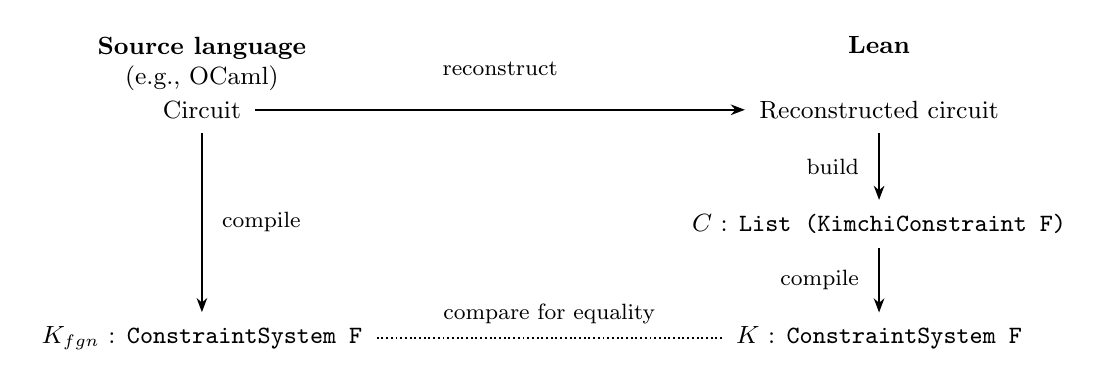
\begin{tikzpicture}[
  artifact/.style={align=center,font=\small,inner sep=5pt},
  heading/.style={align=center,font=\small\bfseries,anchor=north},
  operation/.style={font=\footnotesize,align=center,fill=white,inner sep=2pt},
  flow/.style={-{Stealth[length=1.8mm]},line width=0.6pt},
  comparison/.style={densely dotted,line width=0.7pt}
]
  \node[heading] at (0,1.05)
    {Source language\\{\normalfont(e.g., OCaml)}};
  \node[heading] at (8.6,1.05) {Lean};

  \node[artifact] (circuit) at (0,0) {Circuit};
  \node[artifact] (reconstruction) at (8.6,0) {Reconstructed circuit};
  \node[artifact] (constraints) at (8.6,-1.45)
    {$C$ : \inlinecode{List (KimchiConstraint F)}};
  \node[artifact] (source-system) at (0,-2.9)
    {$K_{fgn}$ : \inlinecode{ConstraintSystem F}};
  \node[artifact] (lean-system) at (8.6,-2.9)
    {$K$ : \inlinecode{ConstraintSystem F}};

  \draw[flow] (circuit.east) --
    node[operation,above=10pt] {reconstruct} (reconstruction.west);
  \draw[flow] (circuit.south) --
    node[operation,right=5pt] {compile} (source-system.north);
  \draw[flow] (reconstruction.south) --
    node[operation,left=5pt] {build} (constraints.north);
  \draw[flow] (constraints.south) --
    node[operation,left=5pt] {compile} (lean-system.north);
  \draw[comparison] (source-system.east) --
    node[operation,above=3pt] {compare for equality} (lean-system.west);
\end{tikzpicture}
\captionsetup{hypcap=false,font=footnotesize,margin=2em}
\captionof{figure}{Compilation of a foreign circuit and its Lean reconstruction,
  compared at the constraint-system level. Equality $K_{fgn}=K$ makes the
  compiler's witness lift applicable to the foreign system.}
\label{fig:compilation-paths}
\end{schematicblock}
\par\addvspace{1.5\baselineskip}

\begin{example}[\href{https://github.com/l-adic/snarky/blob/main/formal/snarky/Snarky/DSL/Bits.lean\#L171}{Four-bit unpacking}]
\label{ex:unpack-lifting}
Let $F$ be either Pasta field and $x$ an input variable. We indicate why
it is easier to work with \texttt{KimchiConstraint}s rather than \texttt{ConstraintSystem}s.
The circuit \inlinecode{unpack x 4} introduces variables $b_0,\ldots,b_3$ and the
intermediate constraints
\[
  C:\quad
  \begin{cases}
    b_i \in \{0,1\} & (i=0,\ldots,3), \\
    x = b_0 + 2b_1 + 4b_2 + 8b_3.
  \end{cases}
\]
Compilation gives the equations
\[
  \begin{array}{@{}rrrr@{}}
    b_0^2-b_0=0 & b_1^2-b_1=0 & b_2^2-b_2=0 & b_3^2-b_3=0 \\
    4b_2+8b_3-t_0=0 & 2b_1+t_0-t_1=0 & b_0+t_1-t_2=0 & t_2-x=0.
  \end{array}
\]
For the isolated gadget with no public inputs, the compiled system $K$ has
the following Generic rows; padding is omitted.\footnote{Matching colors
  identify wiring equivalence classes; $-$ marks unused cells. The variables
  $t_0,t_1,t_2$ are auxiliary.}
{\setlength{\arraycolsep}{3pt}
\renewcommand{\arraystretch}{1.7}
\[
  K:\quad
  \begin{array}{c|ccccccccc|l}
    \text{row} & 0 & 1 & 2 & 3 & 4 & 5 & 6 & \cdots & 14
      & \text{coefficients} \\
    \hline
    0 & \wirecell{wireorange}{b_1} & \wirecell{wireorange}{b_1} & -
      & \wirecell{wireblue}{b_0} & \wirecell{wireblue}{b_0} & - & -
      & \cdots & -
      & [-1,0,0,1,0,-1,0,0,1,0] \\
    1 & \wirecell{wirepurple}{b_3} & \wirecell{wirepurple}{b_3} & -
      & \wirecell{wiregreen}{b_2} & \wirecell{wiregreen}{b_2} & - & -
      & \cdots & -
      & [-1,0,0,1,0,-1,0,0,1,0] \\
    2 & \wirecell{wireorange}{b_1} & \wirecell{wirered}{t_0}
      & \wirecell{wirecyan}{t_1} & \wirecell{wiregreen}{b_2}
      & \wirecell{wirepurple}{b_3} & \wirecell{wirered}{t_0} & -
      & \cdots & -
      & [2,1,-1,0,0,4,8,-1,0,0] \\
    3 & \wirecell{wireblack}{t_2} & - & \wirecell{wiremagenta}{x}
      & \wirecell{wireblue}{b_0} & \wirecell{wirecyan}{t_1}
      & \wirecell{wireblack}{t_2} & - & \cdots & -
      & [1,0,-1,0,0,1,1,-1,0,0]
  \end{array}
\]
}
For any assignment $v$ satisfying $C$, \inlinecode{unpack\_spec} proves
$v(x) = (n : F)$ for some natural number $n < 16$. For the compiled system
$K$, Proposition~\ref{prop:compiler-soundness} gives
\[
  \forall w,\quad w\text{ satisfies }K \Longrightarrow
  \exists n : \mathbb{N},\quad n < 16 \land
    \operatorname{lift}(w)(x) = (n : F).
\]
\end{example}

\section{Pickles applications and reconstruction}
\label{sec:pickles-applications}

Pickles is the recursive proof composition protocol developed at o1Labs to
support the succinct Mina blockchain. It uses Halo-style recursive
composition\footnote{S.~Bowe, J.~Grigg, and D.~Hopwood,
  \href{https://eprint.iacr.org/2019/1021}{\emph{Recursive Proof Composition without a Trusted Setup}},
  Cryptology ePrint Archive, Report 2019/1021, 2019.}
over Kimchi, a PLONKish proof system with custom gates and a Bulletproofs-style
polynomial commitment scheme.\footnote{o1Labs, \emph{Mina book},
  \href{https://o1-labs.github.io/proof-systems/specs/kimchi/}{\textquotedblleft Kimchi\textquotedblright} and
  \href{https://o1-labs.github.io/proof-systems/specs/poly-commitment/}{\textquotedblleft Kimchi Polynomial Commitment\textquotedblright}.}

We reconstruct Pickles applications in Lean by separating their rules'
constraints from their static shape and exporting both, together with the
required parameters.

\subsection{Rules and recursive composition}
\label{sec:rules-composition}

Concretely, Pickles is implemented as a framework in OCaml backed by the Snarky
embedded circuit DSL. The framework user writes their application logic as a
collection of Snarky circuits (called \emph{rules}), and for each rule
(i) designates which inputs are claimed results of a previous rule invocation
and (ii) decides when a proof of that invocation is required.

\begin{example}[\href{https://github.com/l-adic/snarky/blob/main/packages/example/src/Snarky/Example/Transaction/Checked.purs\#L111-L165}{Transaction composition}]
A simplified presentation of Mina's transaction circuit uses two rules.
A statement $a \to b$ asserts a valid transition between ledger states.

\textup{\textbf{Base rule:}} Checks that applying the transaction lawfully transitions the
ledger from state $a$ to state $b$. It depends on no previous rule outputs.

\textup{\textbf{Merge rule:}} Verifies that two transitions $(a \to b)$ and $(b \to c)$
agree on the boundary, resulting in a valid transition $(a \to c)$.
Requires proofs that the two input transitions are valid, either as the
result of a transaction or a prior merge.

\end{example}

The Pickles framework takes the rule declarations and builds the recursive
verification machinery for you. It is implemented over the Pasta cycle of
curves using a technique the framework calls Step/Wrap. The point is that
there is a well-defined boundary:
\begin{boundary}
  \item The author supplies the collection of rules.
  \item Pickles determines the \emph{shape} of the application based on those
    rules (defined below).
  \item Pickles builds the recursive verification machinery based on that
    shape plus the rules' constraint systems, and wires up the application.
  \item Pickles provides a prover and verifier for the resulting application.
    Verifying the correct invocation of a chain of rules is equivalent to
    verifying a single proof plus a few simple scalar identities.
\end{boundary}

One of the insights of this work is that static files exported from a
Pickles application---for example, one written in OCaml---suffice to
reconstruct its Step/Wrap circuits in Lean. Successful certification
provides a certificate establishing properties proved in Lean, which
support the soundness results developed below. Equality of the reconstructed
and original constraint systems allows these results to transfer back to
the original application.

\begin{samepage}
\begin{definition}[\href{https://github.com/l-adic/snarky/blob/main/formal/pickles/PicklesFixture/ApplicationImport.lean\#L130}{Reconstruction}]
\label{def:reconstruction}
Reconstruction builds an application's Step/Wrap circuits in Lean from
exported rules, shape and parameters. A reconstructed application \inlinecode{C}
is \textbf{certified} if it has an
\href{https://github.com/l-adic/snarky/blob/main/formal/pickles/Pickles/Application/CheckedCompile.lean\#L201}{\inlinecode{ApplicationCertified C}}
certificate. The checker
\href{https://github.com/l-adic/snarky/blob/main/formal/pickles/Pickles/Application/CheckedCompile.lean\#L302}{\inlinecode{checkApplication}}
constructs this certificate by checking the circuits' compilation, that
the supplied verification keys correspond to the resulting constraint
systems, and that the embedded verifiers have the required static setup.
\end{definition}
\end{samepage}

\subsection{Shape and reconstruction in Lean}
\label{sec:reconstruction}

We separate the static data---the statement dimensions, number of rules,
and each rule's slot count and sources---from the rules' constraint systems.
This static data is the application's \emph{shape}.\footnote{See
  \href{https://github.com/l-adic/snarky/blob/main/formal/pickles/Pickles/Application/Description.lean}{application shape definitions}
  on GitHub's \inlinecode{main} branch.}
Appendix~\ref{app:reconstruction-types} gives schematic types for this
separation and the resulting reconstruction.

\begin{definition}[\href{https://github.com/l-adic/snarky/blob/main/formal/pickles/Pickles/Application/Description.lean\#L75}{Slot} and \href{https://github.com/l-adic/snarky/blob/main/formal/pickles/Pickles/Application/Description.lean\#L78}{width}]
\label{def:slot-width}
A \textbf{slot} is a port used by the application to hold previous proof
data for its rules.\footnote{Rules may read previous proof statements and
  declare verification requirements, but the framework is responsible for
  wiring slot data to the corresponding rule variables.}
The number of slots declared
by each rule is its \textbf{width}; the maximum of all rule widths is the
application's width. The application's width must not exceed the maximum
supported by the framework, currently 2.
\end{definition}

The application \inlinecode{Shape} records these widths and each rule's slot
sources (i.e., \inlinecode{Self} or which \inlinecode{External} application the slot
references). In other words, it is data that can be represented using
elementary types such as natural numbers or lists of natural numbers.

As a rule $r$ can be represented by a circuit of type
\[
  \mathrm{InputType} \to \mathrm{OutputType}
  \times \prod_{s < \mathtt{nSlots}\,r}
    (\mathrm{Statement}_s \times \mathrm{Bool}),
\]
it can be represented as a series of variable allocations and constraints.
It is not surprising that if you can identify the input, output, and slot
variables correctly, you can compose this rule with an embedded verifier
to process the proof obligations at each slot. The only other values
required to implement the \inlinecode{reconstruct} method are a set of
\inlinecode{Parameters} containing the required verification keys, padding
constants, SRS data, etc. The reconstruction is entirely mechanical.
Figure~\ref{fig:step-wrap-reconstruction} shows the exported rule's place
within the reconstructed Step/Wrap circuits.

\par\addvspace{1.5\baselineskip}
\begin{schematicblock}
\centering
% Panel (a): SVG rows 0--350, cropped from the shared vector PDF.
\includegraphics[width=\linewidth,trim=0 217.5bp 0 0,clip]{build/reconstruction-draft-graphic.pdf}
\end{schematicblock}
\par\addvspace{0.75\baselineskip}
\begin{schematicblock}
\centering
% Panel (b): SVG rows 360--640; keep the caption with this panel.
\includegraphics[width=\linewidth,trim=0 0 0 270bp,clip]{build/reconstruction-draft-graphic.pdf}
\captionsetup{hypcap=false,font=footnotesize,margin=2em}
\captionof{figure}{%
  (a) The application author writes \texttt{Rule}\textsubscript{r}.
  The exporter records its constraints as
  \href{https://github.com/l-adic/snarky/blob/main/formal/pickles/PicklesFixture/Rule.lean\#L36}{\mbox{\texttt{RuleDump shape r}}},
  together with \href{https://github.com/l-adic/snarky/blob/main/formal/pickles/Pickles/Application/Description.lean\#L55}{\texttt{Shape}}
  and \texttt{Parameters}. Lean replays the exported rule constraints (purple)
  and constructs the surrounding
  \href{https://github.com/l-adic/snarky/blob/main/formal/pickles/Pickles/Application/Circuit.lean\#L127}{Pickles verification machinery} (green).
  (b) The shared \href{https://github.com/l-adic/snarky/blob/main/formal/pickles/Pickles/Application/Circuit.lean\#L141}{\texttt{Wrap}}
  circuit is entirely framework-generated and reconstructed from the exported
  shape and parameters.
}
\label{fig:step-wrap-reconstruction}
\end{schematicblock}
\par\addvspace{1.5\baselineskip}

\section{Soundness of recursive verification}
\label{sec:recursive-soundness}

The results below relate the Step/Wrap circuits to
\inlinecode{kimchiVerify} from Section~\ref{sec:wire-verifier}.
They establish the conditional acceptance described in
Section~\ref{sec:recursive-target} and the handover of the remaining
\inlinecode{SgOk} obligations between successive cycles.

\subsection{Step/Wrap verification}
\label{sec:step-wrap-verification}

Fix an application's Step circuit $\mathrm{Step}_r$ for rule $r$ and its
shared Wrap circuit $W$, with Wrap SRS $\sigma$.
Write \href{https://github.com/l-adic/snarky/blob/main/formal/pickles/Pickles/Statement.lean\#L123-L131}{$M_s$}
and \href{https://github.com/l-adic/snarky/blob/main/formal/pickles/Pickles/Statement.lean\#L135-L139}{$M_w$}
for their outgoing messages, and $j(i)$ for slot
$i$'s position in Wrap after padding.
Let $V_s$ and $V_w$ be assignments satisfying the circuit constraints
and the \href{https://github.com/l-adic/snarky/blob/main/formal/pickles/Pickles/Soundness/StepWrap.lean\#L516}{Step/Wrap statement-agreement condition}:\footnote{Since
  $p<q$, canonical representatives in $\mathbb{F}_p$ can be stored unchanged
  in $\mathbb{F}_q$. In the reverse direction, a representative $s$ is stored
  as $(\lfloor s/2\rfloor,\,s\bmod 2)$ in $\mathbb{F}_p\times\{0,1\}$,
  after any protocol shift. Both sides of the equality decode to a
  Step-statement value; the Wrap side uses
  \inlinecode{StepStatement.ofWrap}.}
\[
  \begin{gathered}
    V_s\models C_{\mathrm{Step}_r},
    \qquad V_w\models C_{\mathrm{Wrap}},\\
    \operatorname{decode}_{V_s}(\mathrm{Step}_r.\mathtt{output})
      =\operatorname{decode}_{V_w}(W.\mathtt{stepStatement}).
  \end{gathered}
\]
Then we have the following proposition proven in Lean:

\begin{samepage}
\begin{proposition}[\href{https://github.com/l-adic/snarky/blob/main/formal/pickles/Pickles/Soundness/StepWrap.lean\#L406}{\inlinecode{stepWrap\_kimchiVerify}}]
\label{prop:step-wrap-soundness}
Let $V_s$ and $V_w$ be as above. Let $s_i\in\operatorname{slots}(r)$
have verification key $\mathtt{vk}_i$ and public input $\mathtt{pub}_i$.
Assume \mbox{$V_s(\mathtt{mustVerify}_i)=\mathrm{true}$} and the Lean theorem's
branch-selection, key-binding and setup hypotheses.\footnote{This is a
  schematic statement; the \href{https://github.com/l-adic/snarky/blob/main/formal/pickles/Pickles/Soundness/StepWrap.lean\#L406}{full Lean theorem} gives the branch-selection, key-layout, domain,
  Lagrange-table and SRS hypotheses.}
Then there exists a Kimchi proof $\pi_i$ such that:
\begin{boundary}
  \item The proof components are read from the corresponding $\mathrm{Step_r}$
  and $\mathrm{W}$ cells for slot $i$:
    \[
      \begin{aligned}
        \operatorname{decode}_{V_s}(\mathtt{commitments}_i,\mathtt{opening}_i)
          &= (\pi_i.\mathtt{commitments},\pi_i.\mathtt{opening}),\\
        \operatorname{decode}_{V_w}(\mathtt{evaluations}_i)
          &= \pi_i.\mathtt{evaluations}.
      \end{aligned}
    \]
  \item Let $M_i$ be the Wrap message reconstructed for slot $i$. Then
    \[
      \begin{aligned}
        \pi_i.\mathtt{olds} = \operatorname{zip}\bigl(
          &\operatorname{pad}_{\mathtt{sg}}\bigl(
            \operatorname{decode}_{V_s}(s_i.\mathtt{prevSgs})\bigr),\\
          &\operatorname{pad}_{u}\bigl(
            \operatorname{decode}_{V_w}(M_i.\mathtt{oldBulletproofChallenges})\bigr)\bigr).
      \end{aligned}
    \]
  \item The outgoing messages satisfy
    \[
      \begin{aligned}
        &\operatorname{decode}_{V_s}(M_s.\mathtt{challengePolynomialCommitments}[i])
          = \pi_i.\mathtt{opening.sg},\\
        &\operatorname{decode}_{V_w}(M_w.\mathtt{oldBulletproofChallenges}[j(i)])
          = \mathtt{wireChallenges}(\sigma,\mathtt{vk}_i,\pi_i,\mathtt{pub}_i).
      \end{aligned}
    \]
    The circuits constrain the message digests in their public statements.
  \item If the deferred commitment equation holds, $\pi_i$ verifies according to the
  wire protocol:
    \[
      \mathtt{SgOk}(\sigma,\mathtt{vk}_i,\pi_i,\mathtt{pub}_i)
      \;\Longrightarrow\;
      \mathtt{kimchiVerify}(\sigma,\mathtt{vk}_i,\pi_i,\mathtt{pub}_i)
        =\mathrm{true}.\qedhere
    \]
\end{boundary}
\end{proposition}
\end{samepage}

There is a dual theorem
\href{https://github.com/l-adic/snarky/blob/main/formal/pickles/Pickles/Soundness/WrapStep.lean\#L471}{\inlinecode{wrapStep\_kimchiVerify}}
for the Wrap~$\to$~Step cycle.


Proposition~\ref{prop:step-wrap-soundness} leaves one deferred commitment
equation for each required proof $\pi_i$. Write
\[
  A_i = \bigl(\pi_i.\mathtt{opening.sg},\,
    \mathtt{wireChallenges}(\sigma,\mathtt{vk}_i,\pi_i,\mathtt{pub}_i)\bigr).
\]
The strategy is to carry these accumulators $A_i$ as the old accumulators
of a single proof of the current Wrap circuit. Acceptance of that proof
then discharges all these obligations, under the assumed accumulator
soundness.\footnote{Our assumption of Kimchi soundness includes soundness
  of the underlying IPA protocol.}
Section~\ref{sec:handover} establishes that the circuits enforce this
connection through successive Step/Wrap iteration.

\subsection{Handover theorems}
\label{sec:handover}

Fully establishing that proof obligations are fulfilled---including the
group and scalar identities and the correct propagation of
accumulators---requires treating two successive Step/Wrap runs. A single
run is insufficient. We call these the \textbf{handover results}.

Take upstream and downstream Step/Wrap pairs with assignments $(V_s,V_w)$ and
$(V'_s,V'_w)$, satisfying the respective circuit constraints and the
statement-agreement condition of
Section~\ref{sec:step-wrap-verification}. Fix a required slot $s'_j$ of the
downstream pair whose source is the upstream application. Let $\pi'_j$,
$\mathtt{vk}'_j$, and $\mathtt{pub}'_j$ denote the proof, key, and public
input at slot $j$, as in Proposition~\ref{prop:step-wrap-soundness}, i.e.
\[
  \begin{aligned}
    \pi'_j.\mathtt{commitments}
      &= \operatorname{decode}_{V'_s}(\mathtt{commitments}_j),\\
    \pi'_j.\mathtt{opening}
      &= \operatorname{decode}_{V'_s}(\mathtt{opening}_j),\\
    \pi'_j.\mathtt{evaluations}
      &= \operatorname{decode}_{V'_w}(\mathtt{evaluations}_j),\\
    \pi'_j.\mathtt{olds}
      &= \operatorname{zip}\bigl(
        \begin{aligned}[t]
          &\operatorname{pad}_{\mathtt{sg}}\bigl(
            \operatorname{decode}_{V'_s}(s'_j.\mathtt{prevSgs})\bigr),\\
          &\operatorname{pad}_{u}\bigl(
            \operatorname{decode}_{V'_w}(M'_{w,j}.\mathtt{oldBulletproofChallenges})\bigr)\bigr),
        \end{aligned}
  \end{aligned}
\]
where $M'_{s,j}$ and $M'_{w,j}$ are the Step and Wrap messages
reconstructed for slot $j$.
Fix a required slot $i$ of the upstream pair, and assume the hypotheses of
Proposition~\ref{prop:step-wrap-soundness} at slots $i$ and $j$.
Assume \mbox{$\mathtt{pub}'_j=\restrict{V_w}{\mathrm{public}}$}.
Assume also that slot $j$ has the upstream application's width and statement
size, and that its proof mask keeps a suffix of the padded predecessor
entries. These compatibility conditions and the public-statement equality
form \href{https://github.com/l-adic/snarky/blob/main/formal/pickles/Pickles/Soundness/Handover.lean\#L847}{\inlinecode{StepWrapRun.Hands}}.

\begin{samepage}
\begin{proposition}[\href{https://github.com/l-adic/snarky/blob/main/formal/pickles/Pickles/Soundness/Handover.lean\#L982}{\inlinecode{StepWrapRun.handover\_or\_collision}}]
\label{prop:wrap-handover}
Under these hypotheses, Proposition~\ref{prop:step-wrap-soundness} gives
\[
  \mathtt{SgOk}(\sigma,\mathtt{vk}_i,\pi_i,\mathtt{pub}_i)
  \;\Longrightarrow\;
  \mathtt{kimchiVerify}(\sigma,\mathtt{vk}_i,\pi_i,\mathtt{pub}_i)
    =\mathrm{true}.
\]
Assume additionally that
\[
  \mathtt{kimchiVerify}(\sigma,\mathtt{vk}'_j,\pi'_j,\mathtt{pub}'_j)
    =\mathrm{true}.
\]
Then either a message hash collides, or the complete messages agree and
\[
  \mathtt{kimchiVerify}(\sigma,\mathtt{vk}_i,\pi_i,\mathtt{pub}_i)
    =\mathrm{true}
  \quad\lor\quad
  \mathtt{AccumulatorFailure}(\sigma,\mathtt{vk}'_j,\pi'_j,\mathtt{pub}'_j).\qedhere
\]
\end{proposition}
\end{samepage}

Proposition~\ref{prop:step-wrap-soundness} identifies the upstream proof's
accumulator $A_i$ with the outgoing message entries, and the downstream
proof's old accumulators with the entries reconstructed at slot $j$.
The handover argument combines these identities with \inlinecode{Hands}:
unless a message hash collides, the complete messages agree,\footnote{The
  Wrap messages are compared with their prescribed challenge padding.}
\[
  \begin{aligned}
    &\operatorname{decode}_{V_s}(M_s)
      =\operatorname{decode}_{V'_s}(M'_{s,j})\\
    &{}\land\operatorname{decode}_{V_w}(M_w)
      =\operatorname{decode}_{V'_w}(M'_{w,j}).
  \end{aligned}
\]
Hence
\[
  \forall\,i,\quad V_s(\mathtt{mustVerify}_i)=\mathrm{true}
  \;\Longrightarrow\; A_i \in (\pi'_j).\mathtt{olds}.
\]
Acceptance of $\pi'_j$ supplies the deferred equation for $\pi_i$
unless $\pi'_j$ exhibits \inlinecode{AccumulatorFailure}.
Proposition~\ref{prop:step-wrap-soundness} then gives verification of $\pi_i$.

Since $j$ and $\pi'_j$ stay fixed as $i$ ranges over the upstream pair's
required slots, the same accepted proof discharges all their obligations,
unless a message hash collides or $\pi'_j$ exhibits
\inlinecode{AccumulatorFailure}.

The dual theorem
\href{https://github.com/l-adic/snarky/blob/main/formal/pickles/Pickles/Soundness/Handover.lean\#L732}{\inlinecode{WrapStepRun.handover\_or\_collision}}
establishes the corresponding handover for Step proofs.

\subsection{Terminal verification}
\label{sec:terminal-verification}

A Pickles computation always ends with a Wrap proof. Let $\pi_W$ be a proof
of the downstream Wrap circuit from Section~\ref{sec:handover}, carrying the
outgoing accumulators $A'_j$ for the required proofs $\pi'_j$ consumed by
the downstream Step. Under the existing hypotheses and cryptographic assumptions,
\[
  \pi_W\text{ verifies}
  \;\Longrightarrow\; A'_j\text{ is valid}
  \;\Longrightarrow\; \pi'_j\text{ verifies}
  \;\Longrightarrow\; \pi_i\text{ verifies}.
\]
The last two implications are Sections~\ref{sec:step-wrap-verification}
and~\ref{sec:handover}. Terminal verification must also complete the
outstanding scalar work for the downstream Step proof and bind the
accumulators carried by $\pi_W$ to this execution.

For an application $A$, let \href{https://github.com/l-adic/snarky/blob/main/formal/pickles/Pickles/Application/Terminal.lean\#L360}{\inlinecode{d : TerminalData A}} contain the carried scalar data,
application statement and Step/Wrap message data. It determines the Wrap
public input \inlinecode{d.statement} and the padded accumulator list
\inlinecode{d.wrapAccumulators}. The predicate
\href{https://github.com/l-adic/snarky/blob/main/formal/pickles/Pickles/Application/Terminal.lean\#L471}{\inlinecode{d.Checks}}
requires that the carried scalar claims agree with their recomputed values.
It also requires that the carried Step commitment $\mathtt{sg}$ equal
the commitment to its challenge polynomial.

\begin{proposition}[\href{https://github.com/l-adic/snarky/blob/main/formal/pickles/Pickles/Application/Terminal.lean\#L918}{\inlinecode{terminal\_requiredProofs}}]
\label{prop:terminal-verification}
Let $A$ be a certified application in the sense of
Section~\ref{sec:application-certificate}, with Step and Wrap SRSs
$\sigma_S,\sigma_W$ and Wrap key $\mathtt{vk}_W$. Suppose
\[
  \begin{gathered}
    \mathtt{kimchiVerify}(\sigma_W,\mathtt{vk}_W,\pi_W,d.\mathtt{statement})
      =\mathrm{true},\\
    d.\mathtt{Checks},\\
    \pi_W.\mathtt{olds}=d.\mathtt{wrapAccumulators}.
  \end{gathered}
\]
Assume no hash collisions, \inlinecode{AccumulatorFailure}, or
\inlinecode{KimchiFailure}. Then there exist a branch $r'$ and a connected pair of assignments
$(V'_s,V'_w)$ such that
\[
  \begin{gathered}
    V'_w(\mathtt{whichBranch})=r',\\
    V'_s\models C_{\mathrm{Step}_{r'}},\\
    V'_w\models C_{\mathrm{Wrap}},\\
    \restrict{V'_w}{\mathrm{public}}=d.\mathtt{statement}
  \end{gathered}
\]
and, for the slot proofs decoded as in Proposition~\ref{prop:step-wrap-soundness},
\[
  \forall j,\quad V'_s(\mathtt{mustVerify}_j)=\mathrm{true}
  \;\Longrightarrow\;
  \mathtt{kimchiVerify}(\sigma_W,\mathtt{vk}'_j,\pi'_j,\mathtt{pub}'_j)
    =\mathrm{true}.\qedhere
\]
\end{proposition}

Terminal verification requires two full MSMs: one to check the remaining
Step accumulator, and one as part of verifying the final Wrap proof. It
also performs the deferred Step scalar checks, though no subsequent Step
circuit is run.

\section{Certified applications}
\label{sec:certified-applications}

The capstone theorems of Section~\ref{sec:recursive-soundness} require
numerous hypotheses about slot wiring and message passing between
successive Step/Wrap circuits. For an arbitrary collection of circuits,
listing these hypotheses and proving that they hold would be a nightmare.
The application construction outlined above establishes these structural
properties uniformly from the shape and parameters. \href{https://github.com/l-adic/snarky/blob/main/formal/pickles/Pickles/Application/CheckedCompile.lean\#L201}{\inlinecode{ApplicationCertified}} adds checked
compilation, correspondence of the supplied verification keys, and the
embedded verifiers' static setup. Together they supply the hypotheses
needed to apply the capstones to the reconstructed application.

\subsection{The application certificate}
\label{sec:application-certificate}

Fix a foreign Pickles application $A_{fgn}$ and its Lean reconstruction $A$
in the sense of Section~\ref{sec:reconstruction}. For each circuit
\mbox{$c\in\{\mathrm{Step}_r\mid r\}\cup\{\mathrm{Wrap}\}$}, write $C_c$ for its
intermediate constraints and $K_c$ for its \emph{Lean-compiled} constraint
system. Write $\mathtt{vk}_c$ for the supplied verification key and
$\sigma_c$ for the corresponding SRS.

\begin{definition}[\href{https://github.com/l-adic/snarky/blob/main/formal/pickles/Pickles/Application/CheckedCompile.lean\#L201}{\inlinecode{ApplicationCertified}}]
\label{def:application-certified}
A certificate $\mathtt{cert}:\mathtt{ApplicationCertified}\;A$ contains:
\begin{boundary}
  \item A checked compilation to $K_c$ for each circuit $c$, supplying the
    fixed lift of Proposition~\ref{prop:compiler-soundness}:
    \[
      w\models K_c\ \Longrightarrow\
      \operatorname{lift}_c(w)\models C_c
      \ \land\ \restrict{\operatorname{lift}_c(w)}{\mathrm{public}}
        =\restrict{w}{\mathrm{public}}.
    \]
  \item A proof that each supplied key $\mathtt{vk}_c$ commits to $K_c$
    under $\sigma_c$, with the required public-input and accumulator counts.
  \item The static setup required by the embedded verifiers: correspondence
    of their Lagrange tables to the SRSs, and the required nondegeneracy of
    commitments and correction sums.
\end{boundary}
\end{definition}

The first item lifts satisfying matrices; the second supplies the key
correspondence required by Proposition~\ref{prop:witness-or-failure}.
Combining these gives acceptance-to-assignment lifting with the same
\inlinecode{KimchiFailure} alternative.

\begin{proposition}[\href{https://github.com/l-adic/snarky/blob/main/formal/pickles/Pickles/Application/ProofCorrectness.lean\#L35}{\inlinecode{step\_valuation\_or\_failure}}, \href{https://github.com/l-adic/snarky/blob/main/formal/pickles/Pickles/Application/ProofCorrectness.lean\#L56}{\inlinecode{wrap\_valuation\_or\_failure}}]
\label{prop:acceptance-lifting}
For a certified application, each circuit $c$, proof $\pi$ and encoded
public statement $\mathtt{pub}$,
\[
  \begin{aligned}
    &\mathtt{kimchiVerify}(\sigma_c,\mathtt{vk}_c,\pi,\mathtt{pub})
      =\mathrm{true}\\
    &\quad\Longrightarrow\quad
      \begin{aligned}[t]
        &\bigl(\exists V,\;V\models C_c\ \land\
          \restrict{V}{\mathrm{public}}=\mathtt{pub}\bigr)\\
        &{}\lor\
          \mathtt{KimchiFailure}(\sigma_c,K_c,\mathtt{vk}_c,\pi,\mathtt{pub}).\qedhere
      \end{aligned}
  \end{aligned}
\]
\end{proposition}

This proposition reduces acceptance to circuit satisfaction or Kimchi
failure. It places no bound on the failure event and makes no claim of
witness extraction.

At the application level,
\href{https://github.com/l-adic/snarky/blob/main/formal/pickles/Pickles/Application/ProofCorrectness.lean\#L26}{\inlinecode{SomeKimchiFailure}}
existentially hides which index, key and proof failed at the fixed SRS.
The failure model is that of Section~\ref{sec:kimchi-failure}.

When satisfying matrices are supplied directly, \href{https://github.com/l-adic/snarky/blob/main/formal/pickles/Pickles/Application/MatrixRun.lean\#L115}{\inlinecode{ApplicationCertified.lift\_step}} and \href{https://github.com/l-adic/snarky/blob/main/formal/pickles/Pickles/Application/MatrixRun.lean\#L135}{\inlinecode{lift\_wrap}}
give their satisfying assignments through the fixed compiler lifts.
Those lifts also determine the internal readings of proof components and
messages. Independent equality with foreign constraint systems, when
available as in Section~\ref{sec:compilation}, transfers the same results
to their witness matrices. The certificate itself concerns the reconstructed
circuits and supplied keys; the executable also checks equality with the
foreign constraint systems (Section~\ref{sec:executable-certification}).

\subsection{Step/Wrap verification}
\label{sec:application-step-wrap}

\href{https://github.com/l-adic/snarky/blob/main/formal/pickles/Pickles/Application/Circuit.lean\#L127}{\inlinecode{Circuits.stepCircuit}}
and \href{https://github.com/l-adic/snarky/blob/main/formal/pickles/Pickles/Application/Circuit.lean\#L141}{\inlinecode{Circuits.wrapCircuit}}
build the Step/Wrap circuits of Proposition~\ref{prop:step-wrap-soundness}
with the rules and configuration fixed by $A$.
Fix $\mathtt{cert}:\mathtt{ApplicationCertified}\;A$.
The application's
\href{https://github.com/l-adic/snarky/blob/main/formal/pickles/Pickles/Application/Description.lean\#L55}{\inlinecode{Shape}},
\href{https://github.com/l-adic/snarky/blob/main/formal/pickles/Pickles/Application/Wiring.lean\#L74}{\inlinecode{BackendValid}},
and \href{https://github.com/l-adic/snarky/blob/main/formal/pickles/Pickles/Application/Wiring.lean\#L90}{\inlinecode{Wiring}}
supply the width bounds and key-layout proofs;
its wiring lemmas establish the corresponding padded Wrap position and
source domain for each Step slot. Specializing Proposition~\ref{prop:step-wrap-soundness} to these
constructions therefore discharges these hypotheses uniformly.
The certificate's \href{https://github.com/l-adic/snarky/blob/main/formal/pickles/Pickles/Application/CheckedCompile.lean\#L216}{\inlinecode{cert.stepWrapSetup}} also supplies the SRS-dependent setup
for every branch and slot.

We use the record
\href{https://github.com/l-adic/snarky/blob/main/formal/pickles/Pickles/Application/Run.lean\#L60}{\inlinecode{StepWrapLink A r}}
to bundle satisfying Step and Wrap assignments $(V_s,V_w)$ that agree on
the boundary: Wrap's branch index equals $r$, and the assignments satisfy
the statement-agreement condition of Section~\ref{sec:step-wrap-verification}.

\begin{proposition}[\href{https://github.com/l-adic/snarky/blob/main/formal/pickles/Pickles/Application/Verify.lean\#L284}{\inlinecode{StepWrapLink.verifies\_proof}}]
\label{prop:application-step-wrap}
Let $e:\mathtt{StepWrapLink}\;A\;r$, where $A$ is certified, and let $i$ be a slot with
\mbox{$V_s(\mathtt{mustVerify}_i)=\mathrm{true}$}.
If the slot's key cells read its prescribed source key, then
$e.\mathtt{proof}\;i$ satisfies the conclusions of
Proposition~\ref{prop:step-wrap-soundness}.
\end{proposition}

For satisfying witness matrices $w_s,w_w$ of the certified $K_c$, the
certificate supplies these assignments as
\mbox{$V_s=\operatorname{lift}_{\mathrm{Step}_r}(w_s)$} and
\mbox{$V_w=\operatorname{lift}_{\mathrm{Wrap}}(w_w)$}.
Thus the conclusions of Proposition~\ref{prop:application-step-wrap} hold
for satisfying witnesses of the compiled Step/Wrap circuits.\footnote{\href{https://github.com/l-adic/snarky/blob/main/formal/pickles/Pickles/Application/Certification.lean\#L164}{\inlinecode{matrices\_stepWrap}}.}
When these constraint systems equal those exported by the foreign
application, the same result holds for that application.

\subsection{Handover}
\label{sec:application-handover}

Applying Proposition~\ref{prop:wrap-handover} to arbitrary circuits requires
proofs that their internal wiring passes messages and accumulators correctly
between the verification components. Reconstructed applications use the same
Step/Wrap construction, so these properties are proved once, uniformly in
the application's shape and rules. Certification checks the
application-specific static parameters. A newly exported application can
therefore use the handover theorem without a separate proof of its recursive
verification machinery. The connections between the particular executions
remain explicit in
\href{https://github.com/l-adic/snarky/blob/main/formal/pickles/Pickles/Application/Handover.lean\#L94}{\inlinecode{WrapProofHandover}}.

\begin{proposition}[\href{https://github.com/l-adic/snarky/blob/main/formal/pickles/Pickles/Application/Handover.lean\#L148}{\inlinecode{WrapProofHandover.handover\_or\_collision}}]
\label{prop:application-handover}
Let $A$ and $A'$ be certified applications and let
$e:\mathtt{WrapProofHandover}\;A\;A'\;r\;r'\;i\;j$.
Then the conclusions of Proposition~\ref{prop:wrap-handover} hold for $e$,
with the same proof-acceptance premise and failure alternatives.
\end{proposition}

The theorem
\href{https://github.com/l-adic/snarky/blob/main/formal/pickles/Pickles/Application/Certification.lean\#L142}{\inlinecode{matrices\_wrap\_handover}}
gives this result for satisfying witnesses of the compiled circuits.
Equality with the foreign constraint systems transfers the result to the
foreign applications.

\section{Executable certification}
\label{sec:executable-certification}

The \href{https://github.com/l-adic/snarky/blob/main/formal/scripts/certify_application.lean\#L10}{\inlinecode{certify-application}}
executable reads an application exported from a foreign language and
reconstructs its Step/Wrap circuits.

\subsection{Checking the circuits and verifier setup}
\label{sec:certifying-constraint-systems}

It compiles those circuits in Lean and invokes
\href{https://github.com/l-adic/snarky/blob/main/formal/pickles/Pickles/Application/CheckedCompile.lean\#L302}{\inlinecode{checkApplication}}:
\begin{schematicblock}
\begin{lstlisting}[style=schematic]
def checkApplication (C : Circuits D)
    (steps : (b : D.Branch) $\to$ StepCompilation C b)
    (wrap : WrapCompilation C) :
    Except (ApplicationFailure D) (ApplicationCertified C)
\end{lstlisting}
\end{schematicblock}

This checks the supplied verification keys and static verifier setup,
producing the certificate of Section~\ref{sec:certified-applications}.
The key check establishes
\href{https://github.com/l-adic/snarky/blob/main/formal/kimchi/Kimchi/KeyDerivation.lean\#L120}{\inlinecode{KeyCorresponds}}
between each supplied key and its compiled constraint system, which
Proposition~\ref{prop:acceptance-lifting} uses to derive a satisfying
assignment or \inlinecode{KimchiFailure} from proof acceptance.
The executable also compares the exported constraint systems with the
Lean compilations for equality, as in
Figure~\ref{fig:compilation-paths}.\footnote{The comparison uses
  \href{https://github.com/l-adic/snarky/blob/main/formal/pickles/PicklesFixture/ImportedIndices.lean\#L126}{\inlinecode{compareIndices?}};
  \href{https://github.com/l-adic/snarky/blob/main/formal/pickles/PicklesFixture/ImportedIndices.lean\#L134}{\inlinecode{compareIndices?\_eq\_none\_iff}}
  identifies success with equality.}
It reports success only when both checks succeed.

\subsection{The PureScript transaction application}
\label{sec:transaction-certification}

We apply this procedure to the
\href{https://github.com/l-adic/snarky/blob/main/packages/example/src/Snarky/Example/Transaction/Checked.purs}{PureScript example application},
a simplified Mina transaction circuit. Its
\href{https://github.com/l-adic/snarky/blob/main/packages/example/src/Snarky/Example/Transaction/Checked.purs\#L116}{base rule}
checks a ledger transition; its
\href{https://github.com/l-adic/snarky/blob/main/packages/example/src/Snarky/Example/Transaction/Checked.purs\#L139}{merge rule}
composes two transitions and requires proofs of both. The application has
two Step circuits and one shared Wrap circuit.

The PureScript exporter supplies a complete dump of the rules, shape,
parameters and three constraint systems. The executable consumes this dump
directly; \textbf{no handwritten Lean translation of the application is required}.
It reconstructs and certifies the application, then checks that each
Lean-compiled constraint system equals its exported counterpart.

\begin{samepage}
Consequently, satisfying witnesses of these foreign constraint systems
lift to satisfying assignments of the reconstructed circuits. The results
of Section~\ref{sec:certified-applications} then apply to those assignments,
including successive Step/Wrap executions that satisfy the stated
connection conditions.

\begin{remark}
This example illustrates the intended use of this machinery: establishing,
under the stated assumptions, that a particular application written outside
Lean enforces the proof obligations required by the protocol. \textbf{This
establishes neither the correctness of the application's logic nor the
correctness of the host language's Pickles implementation in general}. It
certifies that the particular exported application was correctly
constructed.
\end{remark}
\end{samepage}

\clearpage
\appendix
\section{Reconstruction types}
\label{app:reconstruction-types}

\begin{schematicblock}
\begin{lstlisting}[style=schematic]
-- Schematic types; fixed field encodings are implicit.
type ApplicationInterface =
  { inputType : Type
  , outputType : Type
  , width : $\mathbb{N}$
  }

-- A slot refers to this application or one of its imports.
type SlotSource nImports
  = Self
  | External (importIndex : Fin nImports)
\end{lstlisting}
\end{schematicblock}

\begin{schematicblock}
\begin{lstlisting}[style=schematic]
-- Slot counts and sources are fixed separately for each rule.
type Shape =
  { inputType : Type
  , outputType : Type
  , nImports : $\mathbb{N}$
  , imports : Vector nImports ApplicationInterface
  , nRules : $\mathbb{N}$
  , nSlots : Fin nRules $\to$ $\mathbb{N}$
  , slotSource :
      (rule : Fin nRules)
      $\to$ (slot : Fin (nSlots rule))
      $\to$ SlotSource nImports
  }
\end{lstlisting}
\end{schematicblock}

\begin{schematicblock}
\begin{lstlisting}[style=schematic]
-- Select the statement type and width of a slot's source.
def slotInterface shape rule slot =
  match shape.slotSource rule slot with
  | Self $\to$
      { inputType = shape.inputType
      , outputType = shape.outputType
      , width = $\max_{\mathtt{rule}<\mathtt{shape.nRules}}$ (shape.nSlots rule)
      }
  | External importIndex $\to$
      shape.imports[importIndex]
\end{lstlisting}
\end{schematicblock}

\begin{schematicblock}
\begin{lstlisting}[style=schematic]
-- Keys and protocol data used by the circuit constructors.
type Parameters shape =
  { wrapKey : WrapKey
  , ruleStepKeys : Vector shape.nRules StepKey
  , stepChunks : $\mathbb{N}$
  , imports :
      Vector shape.nImports
        { wrapKey : WrapKey
        , stepChunks : $\mathbb{N}$
        , stepDomains : List $\mathbb{N}$
        }
  , srs : SRS$_{\mathrm{Pallas}}$ $\times$ SRS$_{\mathrm{Vesta}}$
  , padding : PaddingConstants
  }
\end{lstlisting}
\end{schematicblock}

\begin{schematicblock}
\begin{lstlisting}[style=schematic]
-- Record the rule's operations and returned expressions.
type RuleDump shape rule =
  { operations : List (Allocate $\mathbb{N}$ | Constrain Constraint$_{\mathbb{F}_p}$)
  , output : shape.outputType
  -- Each slot's statement type depends on its source.
  , prevs :
      $\prod$ (slot : Fin (shape.nSlots rule)),
        { statement :
            (slotInterface shape rule slot).inputType
            $\times$ (slotInterface shape rule slot).outputType
        , mustVerify : Bool
        }
  }
\end{lstlisting}
\end{schematicblock}

\begin{schematicblock}
\begin{lstlisting}[style=schematic]
-- One Step circuit per rule, and one shared Wrap circuit.
-- Step and Wrap use the Pasta fields $\mathbb{F}_p$ and $\mathbb{F}_q$.
type Application shape =
  { stepCircuits :
      (rule : Fin shape.nRules)
      $\to$ shape.inputType
      $\to$ Snarky $\mathbb{F}_p$ (StepStatement shape)
  , wrapCircuit :
      WrapStatement shape
      $\to$ Snarky $\mathbb{F}_q$ Unit
  }
\end{lstlisting}
\end{schematicblock}

\begin{schematicblock}
\begin{lstlisting}[style=schematic]
-- Replay the rules inside the Lean Step/Wrap construction.
-- The resulting application is ready for the Lean compiler.
def reconstruct
  : (shape : Shape)
  $\to$ Parameters shape
  $\to$ ((rule : Fin shape.nRules) $\to$ RuleDump shape rule)
  $\to$ Application shape
\end{lstlisting}
\end{schematicblock}

\end{document}
